% DPF 09 talk on strangeness in nucleon

\documentclass[10pt]{beamer}
\usepackage{amsmath}
\usepackage{mathtools}
\usefonttheme{professionalfonts} % using non standard fonts for beamer
\usefonttheme{serif} % default family is serif

%\documentclass[12pt]{beamerthemeSam.sty}
\usepackage{epsf}
%\usepackage{pstricks}
%\usepackage[orientation=portrait,size=A4]{beamerposter}
\geometry{paperwidth=160mm,paperheight=120mm}
%DT favorite definitions
\def\LL{\left\langle}	% left angle bracket
\def\RR{\right\rangle}	% right angle bracket
\def\LP{\left(}		% left parenthesis
\def\RP{\right)}	% right parenthesis
\def\LB{\left\{}	% left curly bracket
\def\RB{\right\}}	% right curly bracket
\def\PAR#1#2{ {{\partial #1}\over{\partial #2}} }
\def\PARTWO#1#2{ {{\partial^2 #1}\over{\partial #2}^2} }
\def\PARTWOMIX#1#2#3{ {{\partial^2 #1}\over{\partial #2 \partial #3}} }

\def\rightpartial{{\overrightarrow\partial}}
\def\leftpartial{{\overleftarrow\partial}}
\def\diffpartial{\buildrel\leftrightarrow\over\partial}

\def\BI{\begin{itemize}}
\def\EI{\end{itemize}}
\def\BE{\begin{displaymath}}
\def\EE{\end{displaymath}}
\def\BEA{\begin{eqnarray*}}
\def\EEA{\end{eqnarray*}}
\def\BNEA{\begin{eqnarray}}
\def\ENEA{\end{eqnarray}}
\def\EL{\nonumber\\}


\newcommand{\map}[1]{\frame{\frametitle{\textbf{Course map}}
\centerline{\includegraphics[height=0.86\paperheight]{../../map/#1.png}}}}
\newcommand{\wmap}[1]{\frame{\frametitle{\textbf{Course map}}
\centerline{\includegraphics[width=0.96\paperwidth]{../../map/#1.png}}}}

\newcommand{\etal}{{\it et al.}}
\newcommand{\gbeta}{6/g^2}
\newcommand{\la}[1]{\label{#1}}
\newcommand{\ie}{{\em i.e.\ }}
\newcommand{\eg}{{\em e.\,g.\ }}
\newcommand{\cf}{cf.\ }
\newcommand{\etc}{etc.\ }
\newcommand{\atantwo}{{\rm atan2}}
\newcommand{\Tr}{{\rm Tr}}
\newcommand{\dt}{\Delta t}
\newcommand{\op}{{\cal O}}
\newcommand{\msbar}{{\overline{\rm MS}}}
\def\chpt{\raise0.4ex\hbox{$\chi$}PT}
\def\schpt{S\raise0.4ex\hbox{$\chi$}PT}
\def\MeV{{\rm Me\!V}}
\def\GeV{{\rm Ge\!V}}

%AB: my color definitions
%\definecolor{mygarnet}{rgb}{0.445,0.184,0.215}
%\definecolor{mygold}{rgb}{0.848,0.848,0.098}
%\definecolor{myg2g}{rgb}{0.647,0.316,0.157}
\definecolor{abtitlecolor}{rgb}{0.0,0.255,0.494}
\definecolor{absecondarycolor}{rgb}{0.0,0.416,0.804}
\definecolor{abprimarycolor}{rgb}{1.0,0.686,0.0}
\definecolor{Red}           {cmyk}{0,1,1,0}
\definecolor{Grey}           {cmyk}{.7,.7,.7,0}
\definecolor{Blue}          {cmyk}{1,1,0,0}
\definecolor{Green}         {cmyk}{1,0,1,0}
\definecolor{Brown}         {cmyk}{0,0.81,1,0.60}
\definecolor{Black}         {cmyk}{0,0,0,1}

\usetheme{Madrid}


%AB: redefinition of beamer colors
%\setbeamercolor{palette tertiary}{fg=white,bg=mygarnet}
%\setbeamercolor{palette secondary}{fg=white,bg=myg2g}
%\setbeamercolor{palette primary}{fg=black,bg=mygold}
\setbeamercolor{title}{fg=abtitlecolor}
\setbeamercolor{frametitle}{fg=abtitlecolor}
\setbeamercolor{palette tertiary}{fg=white,bg=abtitlecolor}
\setbeamercolor{palette secondary}{fg=white,bg=absecondarycolor}
\setbeamercolor{palette primary}{fg=black,bg=abprimarycolor}
\setbeamercolor{structure}{fg=abtitlecolor}

\setbeamerfont{section in toc}{series=\bfseries}

%AB: remove navigation icons
\beamertemplatenavigationsymbolsempty
\title[Newton's Law of Motion]{
  \textbf {Newton's Law of Motion}\\
%\centerline{}
%\centering
%\vspace{-0.0in}
%\includegraphics[width=0.3\textwidth]{propvalues_0093.pdf}
%\vspace{-0.3in}\\
%\label{intrograph}
}

\author[W. Freeman] {Physics 211\\Syracuse University, Physics 211 Spring 2023\\Walter Freeman}

\date{\today}

\begin{document}

\frame{\titlepage}



\frame{\frametitle{\textbf{Clinic hours this week}}
\large
My availability in the Physics Clinic is a bit limited this week because of other commitments.

\bigskip

You can find me in the Clinic:

\begin{itemize}
	\item Today (Tuesday), 1:30-3:30 pm
%	\item Today (Tuesday), 5:15-6:15 (if possible)
	\item Wednesday, 3-5 pm
%	\item Thursday, 2-4 pm
\end{itemize}
\pause
\bigskip\bigskip
}

\frame{\frametitle{\textbf{Extra assistance}}
\Large	Come to B129E for extra assistance with:
	\normalsize
	
	\bigskip
	\BI
	\item ``Soccer problem'' or ``Football problem'' from Exam 1 and related topics:
	\BI
	\item Today, 1:30 or 3:30
	\item Tomorrow, 6:30
	\EI
	\bigskip
	\item ``Goose problem'' (vectors) or ``dog problem'' (graphs) from Exam 1:
	\BI
	\item Today, 2:00 or 4:00
	\item Tomorrow, 7:00
	\EI
	\bigskip
	\item Solving systems of equations by substitution:
	\BI
	\item Today, 2:30 or 4:30
	\item Tomorrow, 7:30
	\EI
	\EI
	
	\bigskip
	
	We can help anyone with any of these topics at any of these times, but these times are more likely to have a group for you.
}


	



\frame{\frametitle{\textbf{Forces}}
\large
\it
Rational mechanics must be the science of the motions which result from any forces, and of the forces which are required for any motions, accurately propounded and demonstrated. For many things induce me to suspect, that all natural phenomena may depend upon some forces by which the particles of bodies are either drawn towards each other, and cohere, or repel and recede from each other: and these forces being hitherto unknown, philosophers have pursued their researches in vain. And I hope that the principles expounded in this work will afford some light, either to this mode of philosophizing, or to some mode which is more true.

\bigskip
\bigskip
\bigskip

\rm

-Isaac Newton, {\it Philosophiae Naturalis Principia Mathematica} (1687), translated from the Latin by Whewell (1837)

\bigskip
\bigskip
\bigskip
\it

}

\frame{\frametitle{\textbf{Forces}}
\large
\it

Mechanics involves figuring out how things move from knowing the forces that act on them, and figuring out what forces act on them
if we know how they move. I suspect that all physical things involve things exerting forces on each other, and since we don't know
what forces these are, nobody's been able to figure much out. Hopefully someone will read this book and figure this stuff out, either
following my suspicion that it's all forces under the hood ({\rm \bf classical physics!}), or with some deeper understanding of nature
({\rm \bf quantum physics!})



\bigskip
\bigskip
\bigskip

\rm

-Isaac Newton, {\it Philosophiae Naturalis Principia Mathematica}, in modern English

}


  \frame{\frametitle{\textbf{Summary from last time}}
    \Large
    \BI
  \item{Forces: anything that pushes or pulls}
  \item{Forces cause accelerations: $\sum \vec F = m \vec a$}
    \BI
  \item{If $\sum \vec F = 0$, $\vec a = 0$: motion at a constant velocity}
  \EI
  \item{Forces come in pairs: if A pushes on B, B pushes back on A}
  \item{It's the vector sum $\sum \vec F$ that matters}
  \item{Draw force diagrams to keep all of this straight}
    \EI
  }


%   \frame{\frametitle{\textbf{What is a force?}}
%    A force is anything that pushes or pulls something:
%    \BI
%  \item{Gravity: $F = mg$, so $mg = ma \rightarrow a = g$}
%    \BI
%  \item{Gravity pulls down on everything (on Earth) with a force $mg$, called its weight}
%  \item{If something isn't accelerating downward, some other force must balance its weight}
%    \EI
%    \EI
%  }
%
%  \frame{\frametitle{\textbf{What is a force?}}
%    A force is anything that pushes or pulls something:
%    \BI
%  \item{Gravity: $F = mg$, so $mg = ma \rightarrow a = g$}
%  \item{``Normal force'': stops things from moving through each other}
%    \BI
%  \item{Are there normal forces on me right now?}
% \pause
%  \item{However big it needs to be to stop objects from sliding through each other}
%  \item{Directed ``normal'' (perpendicular) to the surface}
%  \item{Really caused by electric force/Pauli exclusion principle}
%    \EI
%    \EI
%  }
%
%
%  \frame{\frametitle{\textbf{What is a force?}}
%    A force is anything that pushes or pulls something:
%    \BI
%  \item{Gravity: $F = mg$, so $mg = ma \rightarrow a = g$}
%  \item{``Normal force'': stops things from moving through each other}
%  \item{Tension: ropes pull on both sides equally}
%    \BI
%  \item{What are the forces in a contest of tug-of-war?}
%    \pause
%  \item{What about the forces on the people?}
%    \EI
%  \item{Friction: a force opposes things sliding against each other}
%    \pause
%  \item{Electromagnetic forces, nuclear forces, radiation pressure...}
%    \pause
%  \item{\color{Red}Acceleration is not a force!}
%  \item{\color{Red}... it's the {\it result} of forces}
%    \EI
%  }
%
%\frame{\frametitle{\textbf{Ask a physicist: static electricity}}
%``Can we bottle it and use it to power a house?'' -- we already do!
%}
%
%\frame{
%\Large
%
%Suppose an object is moving in a straight line at a constant speed. Which number of forces could {\it not} be 
%acting on it?
%
%\BI
%\item A: Zero
%\item B: One
%\item C: Two
%\item D: Three
%\item E: Four
%\EI
%
%\pause
%
%Suppose an object is moving in a circle at a constant speed. Which number of forces could {\it not} be 
%acting on it? (Hint: what is the definition of velocity? Of acceleration?)
%
%\BI
%\item A: Zero
%\item B: One
%\item C: Two
%\item D: Three
%\item E: Four
%\EI
%}
%
%
%  \frame{\frametitle{\textbf{Sample questions}}
%    \BI
%    \Large
%  \item{What forces act on a car?}
%    \pause
%  \item{Which forces are bigger or smaller if it's driving at a constant speed?}
%    \pause
%  \item{Which forces are bigger or smaller if it's slowing down?}
%    \pause
%  \item{A 1000 kg car slows from 20 m/s to a stop over 5 sec. What force is required to do this?}
%
%
%    \pause
%
%\bigskip
%\bigskip
%\bigskip
%\normalsize
%\centerline{(Use $\vec F = m \vec a$ to connect force to acceleration, and then kinematics to connect acceleration to motion)}
%
%    \EI
%  }

\frame{\frametitle{\textbf{An important note}}
\large
\BI
\item{Only {\it real physical things} are forces}
\pause
\item{Acceleration is not a force}
\item{``Net force'' is not a force (it's the sum of them)}
\item{Velocity certainly isn't a force}

\pause
\item{If two things don't touch, or interact by gravity, electricity, etc., they don't
exchange forces}
\pause
\item{``A force is something that can send you to the doctor''}
\EI
}

\frame{\frametitle{\textbf{Questions from homework or last week's recitation?}}

}

 \frame{\frametitle{\textbf{Forces in 2D (and 3D)}}
    \large
    \centerline{Force is a vector; handle it like any other}

\bigskip
\bigskip
\bigskip

    \centerline{One copy of Newton's second law in each direction (per object)}

    \bigskip

    \centerline{ \Large $\vec F = m \vec a \rightarrow {{F_x = m a_x} \choose {F_y = m a_y}}$}

  \bigskip

  \pause


  \bigskip
  \bigskip
  \bigskip


  \normalsize


  Important: When dealing with inclines, choose your axes to align with the incline! ($F_N$ is easy that way)



}
 \frame{\frametitle{\textbf{Forces in 2D (and 3D)}}
    \large
    \centerline{Force is a vector; handle it like any other}

\bigskip
\bigskip
\bigskip

    \centerline{One copy of Newton's second law in each direction (per object)}

    \bigskip

    \centerline{ \Large $\vec F = m \vec a \rightarrow {{F_x = m a_x} \choose {F_y = m a_y}}$}

  \bigskip

  \pause


  \bigskip
  \bigskip
  \bigskip


  \normalsize


  Important: When dealing with inclines, choose your axes to align with the incline! ($F_N$ is easy that way)



}


\frame{\frametitle{\textbf{A problem-solving recipe (remember this!)}}
  \large
\BI
\item{{\color{Red}Accounting:} Draw force diagrams for every object}
  \BI
  \item Choose your coordinate system
\item{Work out components (trigonometry) of vectors in funny directions -- no need for numbers}
  \EI
  \pause
\item{{\color{Red}Physics:} Write down $\sum F = ma$ in each dimension, for each object}
  \pause
\item{{\color{Red}Math:} Put in the stuff you know, solve for the stuff you don't}
  \pause
\item{{\color{Red}Kinematics:} Connect acceleration to motion}
  \EI
\pause

\bigskip
\bigskip

\centerline{It really is this easy; I promise!}
\pause
\centerline{``Ask physics the question, don't tell it the answer''}

}

  \frame{\frametitle{\textbf{Sample questions: dealing with two dimensions}}
    \Large

    A stone hangs from the roof of a car by a string; the car accelerates forward at 3 $\rm m/\rm s^2$.

    \BI
  \item{What happens to the string?}
    \pause
  \item{What angle does the string make with the vertical?}
    \pause
  \item{What is the tension in the string?}
    \EI
  }

 \frame{\frametitle{\textbf{Sample questions: dealing with two dimensions}}
    \Large

    A cart slides down a frictionless track elevated at angle $\theta$; what is its acceleration?

}


\frame{\frametitle{\textbf{A new force: Friction}}
	\large
	\BI
	\item{Friction: stops two surfaces from sliding past each other}
	\item{Can either make things move or make things stop; opposes {\it relative} motion}
	\item{Two types:}
	\BI
	\normalsize
	\item{Static friction: keeps two things that aren't sliding stuck together}
	\item{Kinetic friction: opposes the relative motion of two things sliding}
	\EI
	\EI
	\bigskip
	\bigskip
}

\frame{\frametitle{\textbf{Coulomb's friction model}}
	\large
	\centerline{\bf Friction is really complicated!}
	\BI
	\item{Depends on details of surfaces, molecular forces, etc.}
	\item{No way to create a completely accurate general principle}
	\EI
	
	\bigskip
	\bigskip
	
	\centerline{\bf There are a few general principles, though:}
	\BI
	\item{Friction is higher if the normal force is higher}
	\item{Kinetic friction doesn't depend that much on the speed of travel}
	\EI
	
	\bigskip
	\bigskip
	
	\centerline{\bf Simple model: often pretty close}
	\BI
	\item{Friction depends on a property of the surfaces called the {\color{Red}coefficient of friction} $\mu$}
	\item{Force of kinetic friction = $\mu_k F_N$}
	\item{Max force of static friction = $\mu_s F_N$}
	\EI
}

\frame{\frametitle{\textbf{Friction, a summary}}
	\large
	\BI
	\item Kinetic friction points in whichever direction opposes the relative motion
	\item $F_{f,k} = \mu_k F_N$
	\EI
	\bigskip
	\bigskip
	\BI
	\item Static friction points in whichever direction it needs to in order to keep the objects from sliding
	\item You will need to think carefully about this: the direction can change, 
	depending on other things
	\item Static friction is however big it needs to be to keep the objects from sliding, up to a maximum value:
	\item $F_{f,s,\rm max} = \mu_s F_N$
	\EI
}

\frame{\frametitle{\textbf{Traction}}
	Things like cars and humans use friction between their wheels/feet and the ground 
	to accelerate themselves.
	
	\bigskip
	
	We call this force ``traction''. It can point in either direction, depending on how
	the car is trying to turn its wheels, with the engine, brakes, or so on.
	
	\bigskip
	\pause
	In normal use, though, the piece of the wheel touching the ground does not move.
	
	\bigskip
	This means that the traction force is really {\color{Red}\bf static friction}.
	
	\bigskip
	
	
	So $$F_{\rm trac} < \mu_s F_N,$$ just like for static friction. It points
	either forwards or backwards, depending on what the engine/brakes/bicyclist/etc.
	are doing.
} 


\frame{\frametitle{\textbf{Coefficients of friction}}
	
	\centerline { 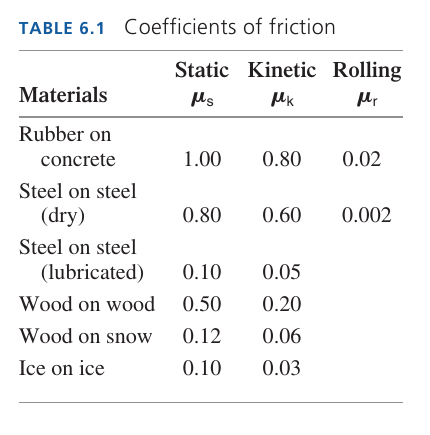
\includegraphics[width=0.5\textwidth]{mu-table.png}}
}


\frame{\frametitle{\textbf{Sample questions}}
	\Large
	What is the fastest possible 0-100 km/hr time for a four-wheel-drive car?
	
	\pause
	\bigskip
	
	What if the car is front-wheel-drive instead?
}
%
%\frame{\frametitle{\textbf{Sample questions}}
%	\Large
%	
%	A block slides down a track elevated at angle $\theta$ with $\mu_k$ known; what is its acceleration?
%}
%


\frame{\frametitle{\textbf{Sample questions}}
	\Large
	An object with mass $m$ on a track is connected by a rope to a hanging weight of mass $M$. The coefficients of friction are $\mu_s$ and $\mu_k$. What is the acceleration of both objects?
	
}






  \frame{\frametitle{\textbf{Sample questions: dealing with multiple objects}}
    \Large

    Two masses of $m_1$ and $m_2$ kg hang from a massless pulley on either side. How do they move?
  }






\frame{\frametitle{\textbf{Summary}}
    \Large
    \BI
  \item{Forces: anything that pushes or pulls}
  \item{Forces cause accelerations: $\sum \vec F = m \vec a$}
    \BI
  \item{If $\sum \vec F = 0$, $\vec a = 0$: motion at a constant velocity}
  \EI
  \item{Forces come in pairs: if A pushes on B, B pushes back on A}
  \item{It's the vector sum $\sum \vec F$ that matters}
  \item{Draw force diagrams to keep all of this straight}
    \EI
  }



  \end{document}

